\graphicspath{{chapters/03/}}
\chapter{Waves of matter}

\section{The Schr\"odinger equation}
Physical laws can never be demonstrated, but only inferred from experiments and then verified or falsified by other ones.


  \subsection{Double-slit experiment}
  The propagation of the electrons in the double-slit experiment has wave-like properties.
  The probability of an electron being detected in certain points of the screen is described by complex-wave amplitudes, which are functions of $x$ and $t$. Being $A(x,y)$ a wave, its intensity:

  $$Intensity(x,t) = A^*(x,t)\cdot A(x,t)$$
\noindent
  The state of the electron in the beams is assumed to be described by a complex amplitude called the wave-function:

  \begin{align*}
    \psi(x,t) &\rightarrow Prob(x,t)\\
              &=\psi^*(x,t)\psi(x,t)\\
              &\equiv |\psi(x,t)|^2
  \end{align*}

  \subsection{Main assumption}
  Electrons behave exactly like photons: they both have a dual particle and wave nature.
  As a consequence, we can assume that for an electron the energy is proportional to frequency:

  $$E = \hbar\omega = h\nu = \frac{p^2}{2m}$$
\noindent
  Protons propagate according to a wave equation:

  $$\biggl(\underbrace{\frac{1}{c^2}}_{\text{speed of light}}\frac{\partial^2{}}{\partial{t^2}} - \nabla^2\biggr)\underbrace{A}_{\text{Maxwell equation}} = 0$$

\noindent
  There is a need to find if the same equation describes the propagation of a massive particle like the electron.
  Let the electron wave particle be:

  $$\psi(x,t) = Ae^{\frac{i}{\hbar}(Et -px)}$$

\noindent
  Then: $\frac{\partial^2{}}{\partial{t^2}}\psi = \omega^2\psi$ and $\frac{\partial^2}{\partial x^2}\psi = p^2\psi$.
  So it is obtained that:

  $${p^2}\propto\underbrace{\omega^2}_{\propto E^2}$$
\noindent
  Then $E = cons|p|$.
  This is true for light, but it is false for massive particles. The correspondence principle implies that:

  $$E = \frac{p^2}{2m}\rightarrow E\propto p^2$$

  And not just to $|p|$.

  \subsection{Defining the Schr\"oedinger equation}
  There is a need to use a different wave equation with respect to the photon's one.
  Noticing that $E^2\propto p^2$ follows from having two time derivatives, we can try a first time derivative to obtain $E\propto p^2$.
  Then the equation to solve becomes:

  $$\biggl(C_1\frac{\partial}{\partial t}-C_2\frac{\partial^2}{\partial x^2}\biggr)\psi = 0$$

  \begin{align*}
    \begin{cases}\frac{\partial\psi}{\partial t} = A\frac{i}{\hbar}E\psi(x,t)\\\frac{\partial^2\psi}{\partial x^2} = A\frac{-1}{\hbar^2}p^2\psi(x,t)\end{cases}\\
    \biggl(C_1\frac{\partial}{\partial t} - C_2\frac{\partial^2}{\partial x^2}\biggr)\psi(x,t) &=0\\
    \biggl(C_1\frac{i}{\hbar}E-C_2\bigl(-\frac{1}{\hbar^2}p^2\bigr)\biggr)\psi(x,t) &= 0\\
    \biggl(C_1\frac{i}{\hbar}E-C_2\bigl(-\frac{1}{\hbar^2}p^2\bigr)\biggr) &= 0\\
  \end{align*}

  Now, considering $\frac{C_1}{C_2}=R\rightarrow \hbar^2$:

  $$\begin{cases} i\underbrace{\hbar\frac{\partial}{\partial t}\psi}_{\text{kinetic energy}}-\frac{\hbar^2}{2m}\frac{\partial^2}{\partial x^2}\psi = 0\\E =\frac{p^2}{2m}\\E = \hbar\omega\end{cases}$$

  Now:

  $$\hbar\omega = E \propto p^2$$
Recall that $\hbar$ is the Dirac's constant, obtained by the following formula: $\hbar=\frac{h}{2\pi}$, where $h$ is Planck's constant.\\
\noindent
  For a free electron, $H$ equals the kinetic energy and is approximately the Hamiltonian.
  For an interacting electron:

  $$H_0 \rightarrow H_0 + \underbrace{V(\vec{r})}_{\text{potential energy}} = H$$
\noindent
  Finally, the Schr\"oedinger equation is:

  $$i\hbar \frac{\partial {}}{\partial {t}}\psi(\vec{r},t) = \biggl(-\frac{\hbar^2}{2m}\nabla^2+V(\vec{r})\biggr)\psi(x,t)$$

    \subsubsection{Quantum Hamiltonian}
    The quantum Hamiltonian can be defined as:

    $$\hat{H} \equiv -\frac{\hbar^2}{2m}\frac{\partial^2}{\partial x}+U(x)$$
\noindent
    Comparing it with a classical Hamiltonian, it can be seen that $\frac{p^2}{2m}\xrightarrow[]{\text{quantization}} - \frac{\hbar^2}{2m}\frac{\partial^2}{\partial x^2}\Rightarrow p^2\rightarrow \hbar^2\frac{\partial^2}{\partial x^2}$.
    Then, due to the fact that the forward propagating wave has a positive momentum, $\hat{p}\rightarrow i\hbar\frac{\partial}{\partial x}$.
    The same happens in three dimensions, where:

    $$i\hbar\frac{\partial }{\partial x}\psi(\vec{x}, t) = \biggl(-\frac{\hbar^2}{2m}\nabla^2+U(\vec{x})\biggr)\psi(\vec{x},t)$$
\noindent
    The Schr\"oedinger equation is then recast as:

    $$i\hbar \frac{\partial {}}{\partial {t}}\psi(\vec{r},t) = \hat{H} \psi(\vec{r},t)$$
\noindent
    To solve this equation there is a need to solve a partial differential equation that defines the state of a system.
    The operators are:

    $$\hat{H} = \biggl(-\frac{\hbar^2}{2m}\nabla^2+U(\vec{r})\biggr)$$

    $$\nabla^2 = \biggl(\frac{\partial^2}{\partial x^2} +\frac{\partial^2}{\partial y^2} + \frac{\partial^2}{\partial z^2}\biggr)$$

\section{Stationary Schr\"oedinger equation}
Assuming that the system conserves mechanical energy:

$$H(p,q, \bcancel{t}) = \frac{p^2}{2m}+U(q,\bcancel{t})$$
\noindent
Considering the plane wave:

$$\psi(\vec{r}, t) = \phi(\vec{r}) e^{-i \frac{E}{\hbar}t}$$
\noindent
By formulating a guess for the form of the solution and plugging it into the Schr\"oedinger equation:

$$E\phi e^{-i \frac{i}{\hbar}(Et)} = He^{-\frac{i}{\hbar}Et}\phi$$
\noindent
Which gives:

$$\hat{H}\phi(\vec{r}) = E\phi(\vec{r})$$
\noindent
Where $E$ is unknown.
This is an eigen problem: given $\hat{H}$, a function $\psi(\vec{r})$ has to be found such that $\hat{H}\psi(\vec{r})$ is a function proportional to $\psi(\vec{r})$ through some constant $E$.
In other words, the energy of a quantum system is an eigenvalue of the quantum Hamiltonian operator.
Energy quantization is obtained and:

$$E = \underbrace{E_0}_{\text{ground state energy}} < \underbrace{E_1 < \cdots < E_n}_{\text{excited state energies}}$$
\noindent
And:

\begin{align*}
  \hat{H}\psi(\vec{r}) &= E_0\psi_0(\vec{r})\\
  \hat{H}\psi(\vec{r}) &= E_1\psi_1(\vec{r})\\
                       &\vdots\\
  \hat{H}\psi(\vec{r}) &= E_n\psi_n(\vec{r})\\
\end{align*}

\section{Ground state of the quantum harmonic oscillator}
The quantum Hamiltonian for the quantum harmonic oscillator is:

$$\hat{H} = - \frac{\hbar^2}{2m}\frac{d{^2}}{d{x^2}} +\frac{1}{2}m\omega^2 x^2$$
\noindent
The solution for the ground state should be in the form $\hat{H}\psi_0 = E$.
\begin{figure}[h!]
    \centering
    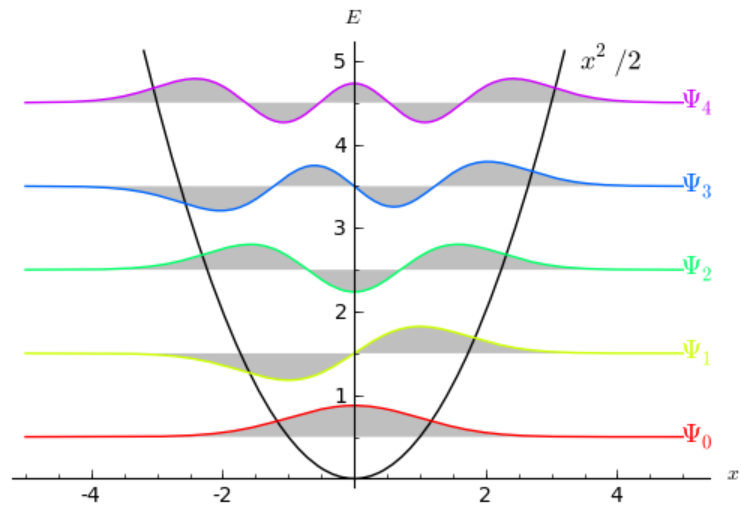
\includegraphics[clip, width=0.6\textwidth]{qm_oscillator.png}
    \caption{\label{fig:qm_oscillator} Quantum mechanics oscillator }
\end{figure}
  \subsection{Form of the ground state}
  The ground state will be in the form:

  $$\psi(x) = \mathcal{N}e^{-\frac{\alpha x^2}{4}}$$

  So:

  \begin{align*}
    -\frac{\hbar^2}{2m}\frac{d{^2}}{d{x^2}}\phi_0 &= -\frac{\hbar^2}{2m}\mathcal{N}\frac{d{}}{d{x}}\biggl[-\frac{\alpha}{2}xe^{-\frac{\alpha x^2}{4}}\biggr]=\\
                                                  &= -\frac{\hbar^2}{2m}\biggl[-\frac{\alpha}{2}e^{-\frac{\alpha x^2}{4}}+\frac{\alpha^2}{4}x^2e^{-\frac{\alpha x^2}{4}}\biggr]\mathcal{N}
  \end{align*}

  So:

  \begin{align*}
    \hat{H}\phi_0 &= -\frac{\hbar^2}{2m}\frac{d{^2}}{d{x^2}}\phi_0 + \frac{1}{2}m\omega^2x^2\phi_0=\\
                  &= \frac{\alpha}{4}\frac{\hbar^2}{m}\phi_0 -\frac{\hbar^2\alpha^2}{8m}x^2\phi_0 + \frac{1}{2}m\omega^2x^2\phi_0
  \end{align*}

  For $\phi_0$ to be an eigenstate $\hat{H}\psi_0 = const\cdot\psi_0$, so the dependence on $x^2$ must be cancelled:

  $$-\frac{\hbar^2}{8m}\alpha^2\bcancel{x^2}\bcancel{\phi_0} + \frac{1}{2}m\omega^2\bcancel{x^2}\bcancel{\psi_0} = 0$$

  From this:

  $$\alpha^2 = \frac{4m^2\omega^2}{\hbar^2}\Rightarrow\alpha=\frac{2m\omega}{\hbar}$$

  So the solution is:

  $$\phi_0(x) = \mathcal{N}e^{-\frac{2m\omega}{\hbar}x^2}$$

  \subsection{Solution of the ground state of the quantum mechanic oscillator}
  The one dimensional quantum mechanic oscillator is the most used model:

  $$H = -\frac{\hbar^2}{2m}\frac{\partial^2}{\partial x^2} + \frac{1}{2}m\omega^2x^2$$

  A wave function for a one particle system contains zero nodes for the ground state.
  It is expected that the ground state is different from zero and we assume a Gaussian for a solution:

  $$\phi_0(x) = \mathcal{N} e^{\alpha x^2}$$

  The objective is to compute $\hat{H}\phi_0 = n\phi_0(x)$:

  \begin{align*}
    \hat{H}\phi_0 &= -\frac{\hbar^2}{2m}\frac{\partial^2}{\partial x^2}(\mathcal{N}e^{-\alpha x^2}) = -\frac{\hbar^2}{2m}\frac{\partial}{\partial x}(-2\alpha x e^{-\alpha x^2})\mathcal{N}=\\
                  &=-\frac{\hbar^2}{2m}(-2\alpha e^{-\alpha x^2}+4\alpha xe^{-\alpha x^2})\mathcal{N}=\\
                  &= \frac{\hbar^2}{\bcancel{2}m}\bcancel{2}\alpha\phi_0 -\frac{\hbar^2}{2m}4\alpha^2 x^2\phi_0\\
    \hat{H}\phi_0 &= \underbrace{\frac{\hbar^2}{m}\alpha\phi_0(x)}_{n\phi_0(x)} + \underbrace{\biggl(\frac{1}{2}m\omega^2-\frac{\hbar^2}{m}\alpha^2\biggr)x^2\phi_0(x)}_{\text{depends on }x^2}
  \end{align*}

  The solutions are found for values of $\alpha$ that set to $0$ the part dependent on $x^2$:

  \begin{align*}
    \frac{1}{2}m\omega^2 -\frac{\hbar^2}{m}2\alpha^2 &= 0\\
    \alpha &= \frac{m\omega}{2\hbar}
  \end{align*}

  Therefore the Gaussian is a good solution:

  $$\phi_0(x) = \mathcal{N}e^{-\frac{m\omega^2x}{2\hbar}}$$

    \subsubsection{Normalization evaluation}
    Consider that $\frac{1}{\sigma^2} = \frac{m\omega}{\hbar} \rightarrow \sigma^2 = \frac{\hbar}{2m\omega}\rightarrow \sigma = \sqrt{\frac{\hbar}{2m\omega}}$.
    Then consider:

    $$\mathcal{N}\int_{-\infty}^\infty e^{-\frac{m\omega x^2}{\hbar}}$$

    And solve the Gaussian integral:

    $$\int e^{-\sigma x^2} = \sqrt{2\pi}\sigma$$

    Then:

    \begin{align*}
      \mathcal{N}^2 &= \frac{1}{\int|\phi_0|^2dx} = \frac{1}{(2\pi\sigma)^{\frac{1}{2}}} = \frac{1}{(2\pi\sqrt{\frac{\hbar}{2m\omega}})^\frac{1}{2}}\\
      \mathcal{N} &= \frac{1}{(2\pi\sqrt{\frac{\hbar}{2m\omega}})^{\frac{1}{4}}}
    \end{align*}

    \subsubsection{Compute the average value of kinetic and potential energy}
    Due to the fact that operations are stochastic, the outcome cannot be predicted. We can only compute the probability or the average values.
    Let $\langle U\rangle $ be the average value of the potential energy, then:

    \begin{align*}
      \langle U\rangle  &= \int P_0(x)U(x)dx = \frac{\int dx e^{-\frac{m\omega x^2}{\hbar}}\frac{1}{2}m\omega^2x^2}{\int dx e^{-\frac{m\omega x^2}{\hbar}}} =\\
          &= \frac{1}{2}m\omega^2\underbrace{\langle x^2\rangle }_{\text{variance }\sigma^2} = \frac{1}{2}\bcancel{m}\omega^{\bcancel{2}}\frac{\hbar^2}{2\bcancel{m}\bcancel{\omega}}=\\
          &=\frac{1}{4}\hbar\omega
    \end{align*}

    So considering $E_0 = \frac{1}{2}\hbar\omega$, the energy remains the same, but the potential energy changes stochastically. Then:

    $$E_0 = \langle U\rangle  + \langle T\rangle $$

    In order to compute the kinetic energy, we need to consider that in quantum mechanics anything that can be measured except time is an observable.
    So, starting with classical mechanics, the observable $o(p,q)$ momentum and position, and after quantization and using the position representation:

    \begin{align*}
      O(\underbrace{\hat{p}}_{-i\hbar\vec{\nabla}},\underbrace{\hat{q}}_{\vec{q}}) &\rightarrow \hat{O}\\
      T = \frac{p^2}{2m}&\rightarrow \hat{T} = \frac{\hat{p}^2}{2m} = \frac{(-i\hbar\nabla)^2}{2m} = -\frac{\hbar^2\nabla^2}{2m}\\
      U(q)&\rightarrow \hat{U}
    \end{align*}

    Now considering the orbital angular momentum $\vec{L} =\vec{r}\cdot\vec{p}$:

    $$\begin{vmatrix}i&j&k\\x&y&z\\P_x&P_y&P_z\end{vmatrix}$$

    Then:

    $$L_z = xP_y - yP_x\xrightarrow[]{\text{quantization}}x\biggl(-i\hbar\frac{\partial}{\partial y}\biggr) - y\biggl(-i\hbar\frac{\partial}{\partial x}\biggr)$$

    Now considering $\langle \phi|O|\phi\rangle$ that specifies the state and that is equivalent to $\langle O\rangle$, where:

    $$\langle O\rangle = \frac{\int dx \phi^*(x)(O(x)\cdot\phi(x))}{\int dx\phi^*(x)\phi(x)}$$

    Then:

    \begin{align*}
      \langle\phi|\hat{T}|\phi\rangle &=\frac{\int dx\phi^*(x)(-\frac{\hbar^2}{2m}\frac{\partial^2}{\partial x^2}\phi(x))}{\int dx |\phi(x)|^2 = \frac{1}{4}\hbar^2}=\\
                                      &=e^{-\alpha x^2}\frac{\partial^2}{\partial x^2}e^{-\alpha x^2} = e^{-\alpha x^2}\frac{\partial}{\partial x}(-2\alpha xe^{-\alpha x^2}) =\\
                                      &=e^{-\alpha x^2}(-2\sigma w^{-\alpha x^2}+4\alpha^2x^2e^{-\alpha x^2})= \\
                                      &=-2\alpha|\phi|^2 = 4\alpha^2 x^2|\phi|^2
    \end{align*}

    And so:

    $$\langle\phi|\hat{T}|\phi\rangle = \frac{-\frac{\hbar^2}{2m}\int |\phi(x)|^2dx}{\int|\phi(x)|^2}2\alpha= - \frac{\hbar^2}{2m}4\alpha^2\frac{\int dx|\psi|^2x^2}{\int dx|\psi|^2}$$


\section{Quantum particle in a one dimensional infinite square well}
We previously discussed at the classical level that a physical system can be bound or unbound. In quantum physics, a bound state is a quantum state of a particle subject to a potential such that the particle has a tendency to remain localized in one or more regions of space. Ultimately, matter and life exist because of bound systems, which allow the presence of macro structures.
While trying to solve a bound system problem, we will require a toy model - a model deliberately too simple to be realistic, which is not meant to predict the outcome of an experiment, but rather to understand the qualitative nature of the object under study.
While implementing a toy model, if the scale where a detail occurs is very small compared with the size of the box, its effect can be neglected. As a consequence, everything which occurs within the box is idealized, allowing us to solve the problem. It's all a matter of scale e.g. $\lambda$ is the scale for details, $L$ the size of the physical system, $\eta$ the energy we are interested in, $E$ the unbounding energy. If the ratio $\frac{\lambda}{L}\ll1$ and $\frac{\eta}{E}\ll1$ , we can neglect the detail.\\
\\
\begin{figure}[h!]
    \centering
    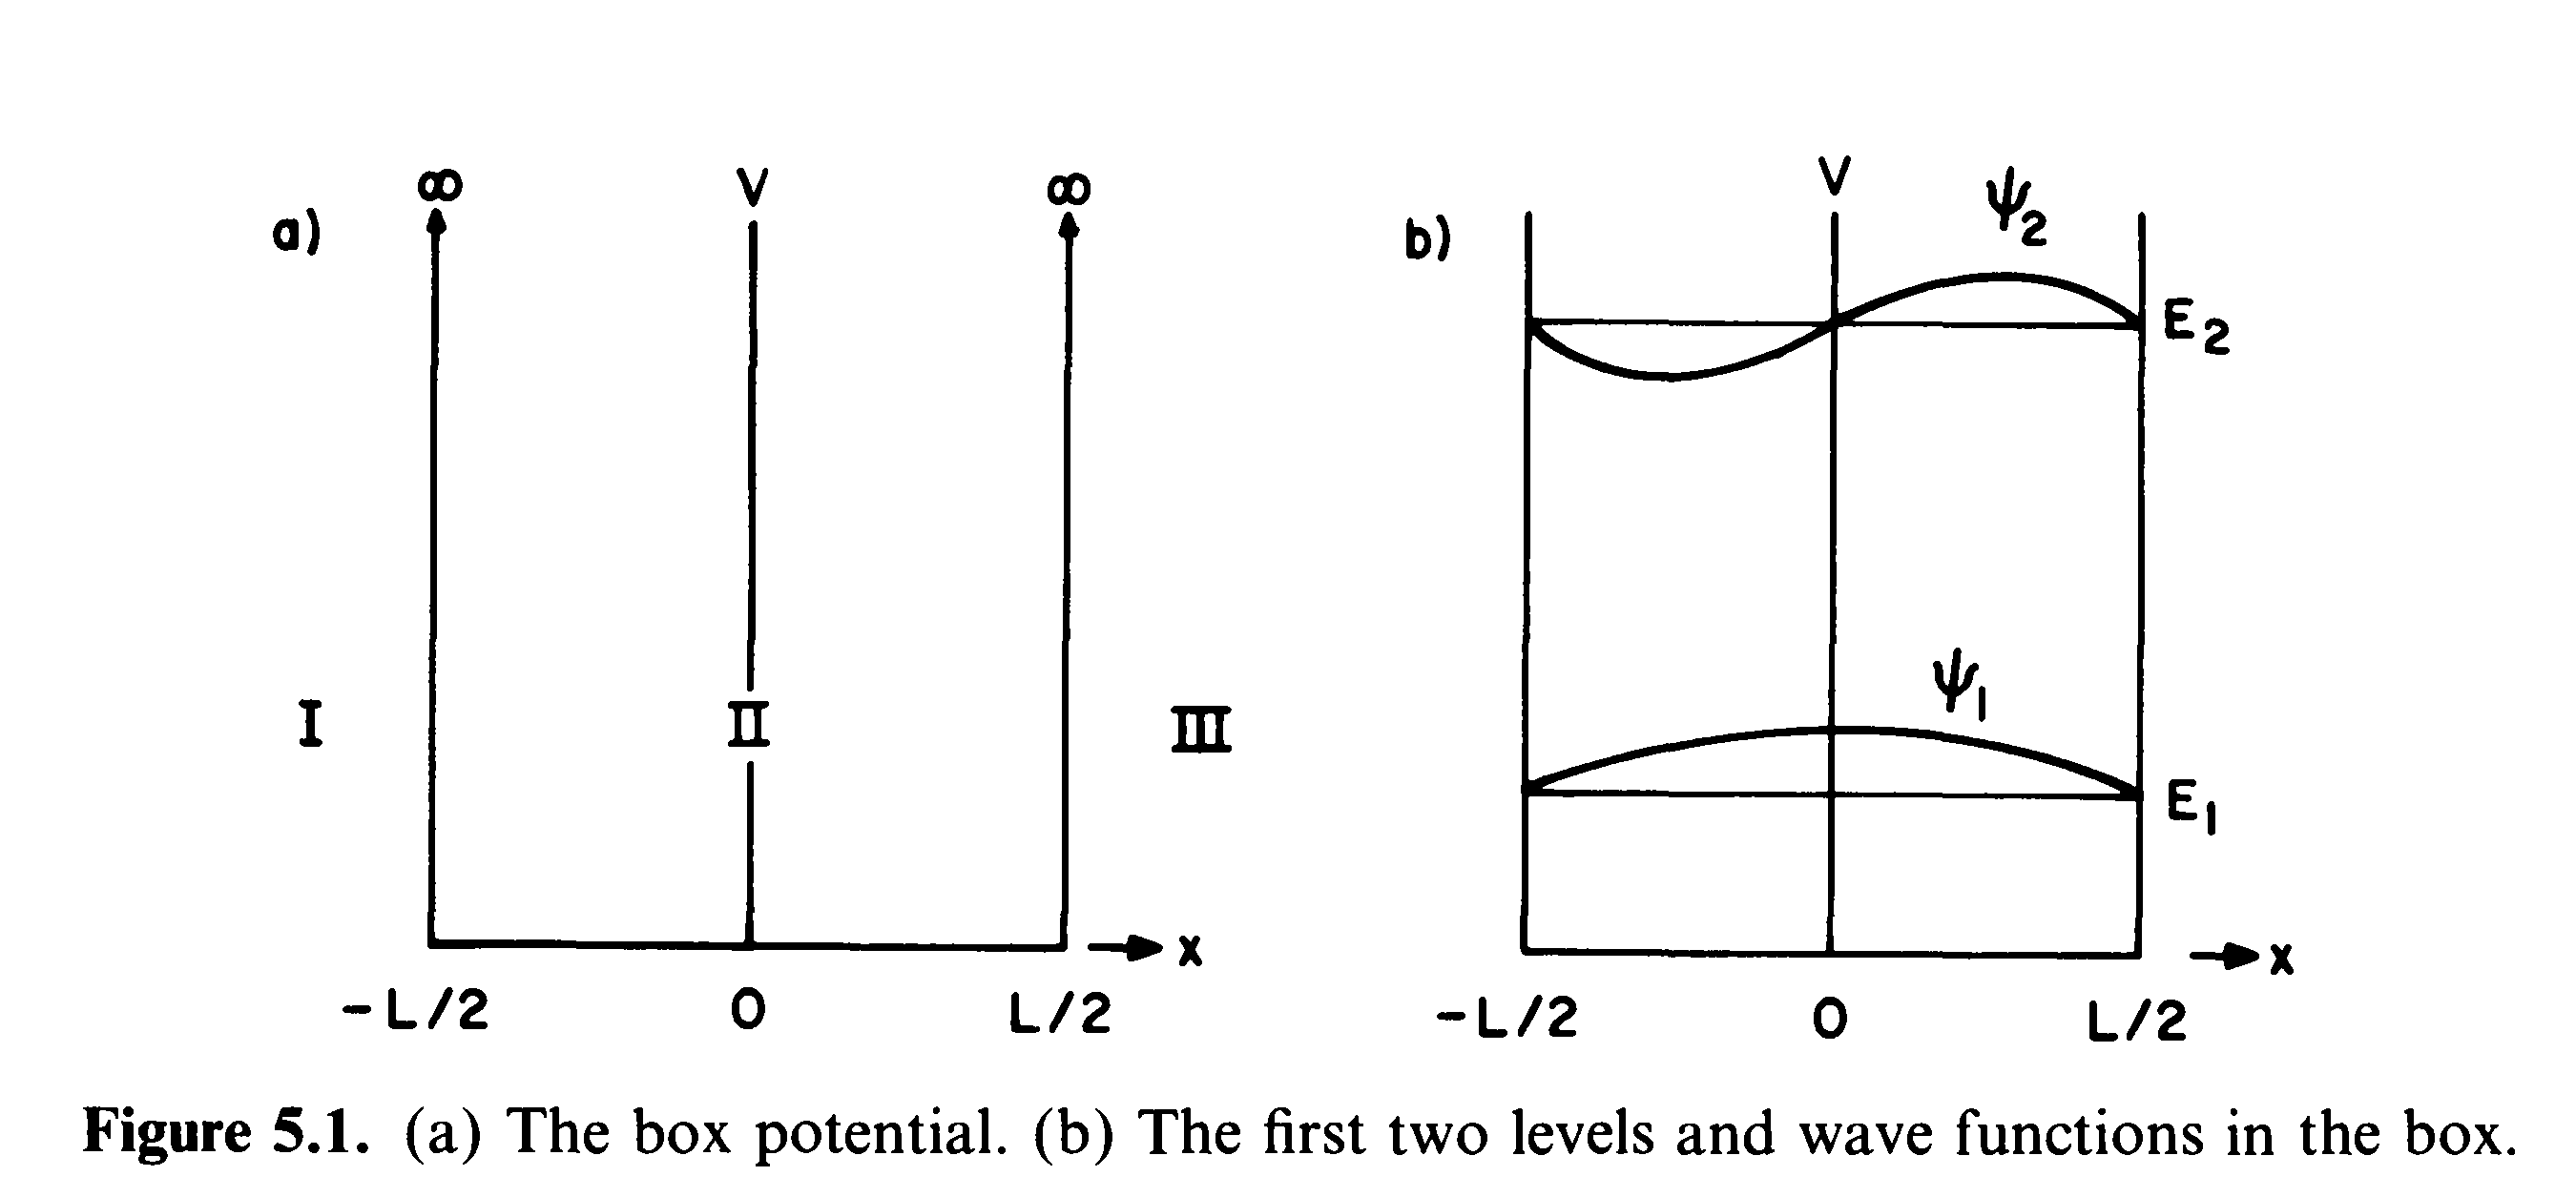
\includegraphics[clip, width=0.6\textwidth]{1D_well.png}
    \caption{\label{fig:1D_well} Particle trapped in 1D infinite square well}
\end{figure}
\noindent
For the case of a quantum particle in a one dimensional infinite square well, we will consider a particle constrained in a trap where interactions are so strong that it cannot escape and with two confining directions much narrower than the third. We can consider a box with size $L/2$ and $-L/2$ and find the eigenvalues and eigenvectors for the Schro\"edinger equation in this specific condition.
This can be modelled with a one dimensional confining potential:

$$U(x) = \begin{cases} 0, &-\frac{L}{2}<x<\frac{L}{2}\\\infty &|x|>\frac{L}{2}\end{cases}$$

Inside the box $U=0$, so the Schr\"oedinger equation is:

$$-\frac{\hbar^2}{2m}\frac{d{^2}}{d{x^2}}\psi(x) = E\psi(x)$$

Mathematically this looks like the Newton's equation for the harmonic oscillator:

$$+m \frac{d{^2}}{d{t^2}}x(t) = -kx(t)$$

Where $x\rightarrow t$ and $\psi\rightarrow x$.
However, the constraints are different. Instead of the classical initial values $x(0) = x_0$ and $\frac{d{}}{d{t}}x|_{t=0} = 0$, there is a boundary value $\psi\bigl(\pm \frac{L}{2}\bigr) = 0$.

  \subsection{Solution}
  Given the mathematical similarity between the two equations, the general structure of the solution should be:

  $$\psi(x) = \begin{cases}A_1\cos k_1 x \\A_2\sin k_2x\end{cases}$$

  Where $A_1,A_2,k_1, k_2$ need to be fixed.

    \subsubsection{Option 1}
    $A_1\cos\biggl(k_1 \frac{L}{2}\biggr) = 0$, then:

    \begin{align*}
      k_1 \frac{L}{2} &=\pm \frac{\pi}{2}\pm n\pi\Rightarrow\\
      \Rightarrow k_1^{(n)} &=\pm \frac{\pi}{L},\pm \frac{3\pi}{L},\dots =\\
                            &= \pm 2(n-1)\frac{\pi}{L}\qquad n = \mathbb{N}
    \end{align*}

    For this option, the possible quantized energy levels are:

    $$E^{(n)} = \frac{\hbar^2}{2m}\frac{\pi^2}{L^2}(2n-1)^2$$

    \subsubsection{Option 2}
    $A_1\sin\biggl(k_2 \frac{L}{2}\biggr) = 0$, then:

    \begin{align*}
      k_2 \frac{L}{2} &=\pm \pi\pm n\pi\Rightarrow\\
      \Rightarrow k_2^{(n)} &=\pm \frac{2\pi}{L},\pm \frac{4\pi}{L},\dots =\\
                            &= \pm 2n\frac{\pi}{L}\qquad n = \mathbb{N}
    \end{align*}

    For this option, the possible quantized energy levels are:

    $$E^{(n)} = \frac{\hbar^2}{2m}\frac{\pi^2}{L^2}(2n)^2$$

    \subsubsection{$A_1$ and $A_2$}
    $A_1$ and $A_2$ can be determined by applying the normalization conditions.
    The probability of finding the particle somewhere in the box is one, so:

    \begin{align*}
      \int_{-\frac{L}{2}}^{\frac{L}{2}} dx|\psi(x)|^2 = 1\\
      1 = \int_{-\frac{L}{2}}^{\frac{L}{2}} dx\begin{cases}A_1^2\cos^2k_1x\\A_2^2\sin^2 k_2x\end{cases}\Rightarrow\begin{cases}A_1 = \\A_2 = \end{cases}
    \end{align*}

    \subsubsection{Summary}
    Summarizing the results:

      \paragraph{Energy spectrum}

      $$E_n = \frac{\hbar^2}{2m}\frac{\pi^2}{L^2}\mathcal{L}^2$$

      \paragraph{Energy eigenstates}
      The energy eigenstates of the stationary wave-functions are:

      $$\psi_m(x) = \begin{cases}A_1\cos k_1 x & n\ odd\\ A_2\sin k_2 x & n\ even\end{cases}$$


  \subsection{Discussion}

    \subsubsection{Quantized momenta}
    From the quantized energy:

    $$E_n = \frac{1}{2m}\biggl(\underbrace{\frac{\pi^2\hbar^2}{L_2}m^2}_{=p_m^2}\biggr)$$

    So the quantized momenta is $p_m = \pm \frac{\pi\hbar}{L}m$.

    \subsubsection{Lowest energy state}
    In classical mechanics, the lowest energy state is $p = 0\Rightarrow E = 0$.
    Differently, in quantum mechanics the lowest energy level is:

    $$E_1 = \frac{\hbar^2}{2m}\biggl(\frac{\pi}{L}\biggr)^2 > 0$$

    Recalling that $E_1 = \frac{p_1^2}{2m}$, it is inferred that:

    $$p_1 = \pm \frac{\hbar\pi}{L}\neq 0$$

    $p_1$ can point in $+$ or $-$ direction with equal probability, so the quantum uncertainty is $\Delta p =\frac{2\hbar\pi}{L}$.
    On the other hand, $\Delta p \sim L$, so there is quantum delocalization for $\psi_1(x)$.
    However in the classical ground state:

    $$T = \frac{p^2}{2m = 0}\Rightarrow p = 0\Rightarrow \Delta p = 0$$

    But $\Delta q = b$, hence there is a violation of the uncertainty principle:

    $$\Delta q\Delta p = 0$$

    \subsubsection{Correspondence principle}
    By considering that for $L\rightarrow\infty$ and $m\rightarrow\infty$ $E_0 = 0$, there is no uncertainty in classical mechanics. In addition, $E_{n+1}-E_n \rightarrow 0$, so there is no quantization.
    As a consequence, classical mechanics is contained in quantum mechanics in the macroscopic limit, for large size and heavy masses.

    \subsubsection{Excited states}
    The wave function of the n-th excited state has $N$ nodes, a general result that holds for any quantum system.

\section{Two dimensional square well}
Consider a quantum particle in a two dimensional square well with dimensions $L_1$ and $L_2$.
Then:

$$\hat{H} = -\frac{\hbar^2}{2m}\frac{\partial {^2}}{\partial {x^2}}-\frac{\hbar^2}{2m}\frac{\partial {^2}}{\partial {y^2}}$$

Any $H$ can be separated as: $H(x,y) = H_1(x) + H_2(y)$.
Anytime the Hamiltonian factorizes, i.e. $\hat{H}=\sum_i{\hat{h}_i}$, the solution of the Schr\"oedinger equation can be written as the product of two wave functions $\phi(x,y)=\phi_1(x)\phi_2(y)$. The corresponding energy will be obtained by summing the two energies $E=E_1+E_2$. By applying this property, we can write the solution to the Hamiltonian for our problem.

  \subsection{Solution}
  Then the solution is:

  $$\begin{cases}\phi(x,y) = \phi_1(x)\phi_2(y)\\H\phi=(E_1+E_2)\phi\end{cases}$$

  Where $H_1\phi_1 = E_1\phi_1$  and $H_2\phi_2 = E_2\phi_2$
  So:

  \begin{align*}
    (H_1 + H_2)\phi_1(x)\phi_2(y) &= H_1\phi_1(x)\phi_2(y) + H_2\phi_1(x)\phi_2(y)=\\
                                  &= \phi_2(y)\hat{H}_1\phi_1(x)+\phi_1(x0+\phi)1(x)H_2\phi_2(y)=\\
                                  &= \phi_2 E_1\phi_1 + \phi_1E_2\phi_2=\\
                                  &=(E_1+E_2)\phi_1\phi_2
  \end{align*}

 Resulting in:

  $$\phi_n(x) = \begin{cases}\sqrt{\frac{2}{L_{x}}} \sin k_n x\\ \sqrt{\frac{2}{L_{x}}} \cos k_n x\end{cases}$$
  $$\phi_m(x) = \begin{cases}\sqrt{\frac{2}{L_{y}}} \sin k_m y\\ \sqrt{\frac{2}{L_{y}}} \cos k_m y\end{cases}$$

  For $n=1$ and $m=1$:

  $$\psi_1 = \sqrt{\frac{2}{L_{x}}\frac{2}{L_{y}} \cos k_1^x x \cos k_1^y y}$$
  $$k_1^x = \frac{\pi}{L_{x}} n = \frac{\pi}{L_{x}}$$
  $$k_1^y = \frac{\pi}{L_{y}} m = \frac{\pi}{L_{y}}$$

  For $n=2$ and $m=1$:
  $$\psi_2 = \sqrt{\frac{2 \cdot 2}{L_{x}L_{y}}} \sin k_2^x x \cos k_1^y y$$

  The total energy can be obtained as $E_{n,m} = E_n^x+E_m^y = -\frac{\hbar^2}{2m}\pi^2\biggl(\frac{n^2}{L_x^2}+\frac{m^2}{L_y^2}\biggr)$.
  Then the ground state is $E_{11} = E_1^x+E_1^y$ and the system is doubly degenerative in opposite directions:

  $$E_{12} + E_1^x+E_2^y + E_{21} = E_2^x+E_1^y$$

\section{Lattice discretization}
Lattice discretization is a technique by which a numerical solution is obtained by exploiting the connection between operators and matrices.\\

\noindent
We know that the wavefunction should be normlized and localized in a certain position of the space. By going towards the end and beginning of the x-axis, the function will go to zero - meaning that we have a maximum and minimum after which the function value can be neglected. We can either stop at maximum/minimum point, and this would be a first approximation. But let us divide the axis into little dots, such that the function can be considered almost constant in each dot. We are going to obtain a very accurate step-wise representation of the function,  and we can proceed until the result is good enough i.e. when the lattice space is smaller than the scale at which the wavefunction changes. Though discretization, we can tune the number of dots required to obtain an accurate result.\\
\\
\noindent
A large but finite number of equally spaced possible position is used. The possible positions are $x = x_{\min} + \Delta x$, where $\Delta x = \frac{x_{\max}-x_{\min}}{N}$.
After discretization, the wave function is represented by a list $\psi(x) \rightarrow(\psi_1,\dots, \psi_N)$.
Thus, the wave function becomes a vector and the Hamiltonian a matrix.

  \subsection{Discrete representation of the derivative}

  $$\frac{d{}}{d{x}}\psi(x) \rightarrow \frac{\psi_{i+1}-\psi_i}{\Delta x}$$

  $$\frac{d{^2}}{d{x^2}}\psi(x) \rightarrow \frac{\psi_{i+1}+\psi_{i-1}-2\psi_i}{\Delta x^2}$$

  Let the Kronecker delta be:

      $$\delta_{ij} =\begin{cases}1 &i=j\\0 &i\neq j\end{cases}\Rightarrow S_{ij} \rightarrow\begin{pmatrix}1 & 0 & \cdots\\\vdots & \ddots &\vdots \\0&\cdots & 1 \end{pmatrix}$$

  Now:

  $$-\frac{\hbar^2}{2m}\frac{d{^2}}{d{x^2}}\rightarrow T_{ij}=-\frac{\hbar^2}{2m\Delta x^2}(\delta_{ij+1}+\delta_{ij-1}-2\delta_{ij})$$

  Indeed:

  $$\sum\limits_{j}T_{ij}\psi_i = -\frac{\hbar^2}{2m}(\psi_{i+1}+\psi_{i-1}-2\psi_i)\frac{1}{\Delta x^2}$$

  Now $V(x) \rightarrow V_{ij} = V_i\delta_{ij}$, so:

  $$\sum\limits_{j}V_{ij}\psi_j = V_i\psi_i$$

  Finally, the matrix lattice representation is obtained as:

  $$H_{ij} = T_{ij} + V_{ij}$$

  $$H_{ij} = \begin{pmatrix}\frac{\hbar^2}{m\Delta x^2} + V_1 & -\frac{\hbar^2}{2m\Delta x} & 0 & \cdots\\ -\frac{\hbar^2}{2m\Delta x^2} & \frac{\hbar^2}{m\Delta x^2}+V_2-\frac{\hbar^2}{2m \Delta x^2} & 0 & \cdots\\ 0 & -\frac{\hbar^2}{2m\Delta x^2} & \frac{\hbar^2}{m\Delta x^2}+V_3 - \frac{\hbar^2}{2m\Delta x^2} & \cdots\end{pmatrix}$$
\noindent
  Solving the matrix eigenproblem $\sum\limits_i H_{ij}\psi_i = E_i\psi_i$ yields $\{E_i\}_{i=\{1,\dots,N\}}$ and $\{y_j\}_i$. \\
  The dimensionality grows with the number of mesh points $N$.
  The exact case is $N\rightarrow\infty$.
  Quantum mechanics is described by an infinite dimensional vector space called the Hilbert space.
\noindent
  After discretization, changing from coordinate representation to momentum representation (and opposite), i.e. performing Fourier transformation, basically involves changing a basis in the vector space that describes the state of the system. Lattice discretization allows us to go from quantum mechanics mathematics to linear algebra.

\section{Time evolution operators}
Consider the time-dependent Schr\"oedinger equation:

$$i\hbar\frac{\partial}{\partial t}\psi(x,t) = \hat{H}\psi(x,t)$$

Where:

$$\psi(x,t) = e^{-\frac{i}{\hbar}\hat{H}(t-t_0)}\psi(x,t_0)$$

And the time-evolution operator:

$$U(t,t_0) = e^{-\frac{i}{\hbar}\hat{H}(t-t_0)}$$

If the argument of the Taylor expansion is too large, we will infinitely many operators - unless it is a special quantum mechanics operators such that it is the eigenvalues of the Hamiltonian.
Let $\vec{a}_k$ be an eigenvector, then:

$$e^{\hat{A}}\vec{a}_k = e^{a_k}\vec{a}_n$$

As a consequence, the time-evolution operator for the eigenvectors of the Hamiltonian can be easily evaluated.
If $\psi(x,t=t_0) = \phi_n(x)$, where $\hat{H}\phi_n(x) = E_n\phi_n(x)$, then:

$$\psi(x,t) = e^{-\frac{i}{\hbar}(t-t_0)E_n}\phi_n(x)$$

And:

$$P(x,t) = |\psi(x,t)|^2 = |e^{-\frac{i}{\hbar}(t-t_0)E_n}|^2|\phi_n(x)|^2$$

If it has a pure phase: $|e^{ia}|^2 = e^{ia}(e^{ia})^* = e^{i(a-a)} = 1$, then:

$$P(x,t) = |\phi_n(x)|^2 = P(x,t_0)$$

And it is the same as the initial time.
